% !TeX spellcheck = en_US
% !TeX encoding = UTF-8

\documentclass[
	paper=A4,
	twoside=true,
	openright,
	parskip=full,
	chapterprefix=true,
	13pt,
	headings=normal,
	bibliography=totoc,
	listof=totoc,
	titlepage=on,
	draft
%	final
	]{scrreprt}

\usepackage{lieb}
\graphicspath{{images/}}

\title{Sensitivity Studies for the Model Unspecific Search}
\date{XX.XX.2017}
\author{Jonas Lieb}

\makeatletter
\let\theauthor\@author
\let\thetitle\@title
\makeatother

\hypersetup{
	pdftex,
	pdfauthor={\theauthor},
	pdftitle={\thetitle},
	pdflang={en-US},
	pdfcreator={},
	pdfproducer={},
}

\begin{document}

\cleardoublepage
\pagenumbering{roman}
\pagestyle{empty}


% !TeX spellcheck = de_DE
% !TeX encoding = UTF-8
% !TeX root = ../document.tex

\makeatletter
\begin{titlepage}
		\tgherosfont
		\centering
		
		\Large
		
		\vspace*{\fill}
		
		{
			\fontsize{30pt}{28pt}\selectfont\bfseries \color{ctcolormain}
			\@title
		}
		
		\vspace{24mm}
		
		\textsf{von} \\
		{\LARGE \@author} \\[32mm]
		
		Masterarbeit im Fach Physik \\[8mm]
		
		\large
		
		\textsf{vorgelegt der} \\
		Fakultät für Mathematik, Informatik und Naturwissenschaften \\der RWTH Aachen \\[8mm]
		
		\textsf{im} \\
		April 2017 \\[8mm]
		
		\textsf{angefertigt am} \\
		III. Physikalischen Institut A \\[8mm]
		
		\textsf{bei} \\
		Prof. Dr. Thomas Hebbeker \\
\end{titlepage}
\makeatother
\cleardoublepage
% !TeX spellcheck = de_DE
% !TeX encoding = UTF-8
% !TeX root = ../document.tex

Ich versichere, dass ich die Arbeit einschließlich beigefügter Darstellungen und Tabellen selbständig angefertigt und keine anderen als die angegebenen Quellen und Hilfsmittel benutzt sowie Zitate kenntlich gemacht habe. 

\vspace{3cm}

\theauthor \\
Aachen, den \germandate
\cleardoublepage

% !TeX spellcheck = en_US
% !TeX encoding = UTF-8
% !TeX root = ../document.tex

%\chapter*{Abstract}
{\usekomafont{chapter}Abstract}
\chapterheadendvskip

In 2015 and 2016, the \acs{CMS} detector recorded proton-proton collisions at an unprecedented center of mass energy of $\sqrt{s} = \SI{13}{\TeV}$. The \acf{MUSiC} provides an automated search for various possible signatures of new physics in these data.

In a three step process, \acs{MUSiC} first classifies events according to the physics content of the final state, searches a set of kinematic distributions for the most significant deviation between \acl{SM} \acl{MC} simulations and observed data and finally applies a statistical hypothesis test to draw conclusions about the presence of new physics in the observed dataset.

In this thesis, the discovery potential towards new physics is assessed. For this purpose, a quantification of the test power is defined. Subsequently, the framework is applied to simulated events of four benchmark models for new physics. Alongside the discovery potential towards these theories, the influence of several existing and newly introduced features and parameters on the sensitivity is measured.

% !TeX spellcheck = de_DE
% !TeX encoding = UTF-8
% !TeX root = ../document.tex

\vspace{1cm}
{\usekomafont{chapter}Kurzdarstellung}
\chapterheadendvskip

\begin{otherlanguage}{german}
In den Jahren 2015 und 2016 wurden vom \acs{CMS}-Experiment Kollisionen von Protonenpaaren bei einer Schwerpunktsenergie von $\sqrt{s} = \SI{13}{\TeV}$ beobachtet. Mithilfe der modellunabhängigen Suche in \acs{CMS} (\ac{MUSiC}) können die aufgezeichneten Daten automatisiert nach Anzeichen neuer Physik durchsucht werden.

Die \ac{MUSiC} Analyse besteht aus einem mehrstufigen Verfahren, bei dem die aufgezeichneten Ereignisse zuerst ihrem Endzustand gemäß in verschiedene Klassen eingeteilt werden. In jeder Klasse werden daraufhin Histogramme einiger kinematischer Variablen aggregiert und die größten Abweichungen zwischen der beobachteten Verteilung und einer Erwartung aus \acl{MC}-Simulationen des Standardmodelles berechnet. Im Rahmen eines statistischen Hypothesentests wird schließlich festgestellt werden, ob beobachtete Daten Hinweise auf neue Physik beinhalten.

In dieser Arbeit wird das Entdeckungspotential der Analyse untersucht. Zu diesem Zweck wird zuerst eine geeignete quantitative Teststärke definiert. Diese wird anschließend für Simulationsergebnisse vier verschiedener Modelle neuer Physik ausgerechnet. Neben dem absoluten Wert in Bezug auf diese Modelle wird der Einfluss verschiedener Funktionalitäten und Parameter auf die Sensitivität untersucht.
\end{otherlanguage}
\cleardoublepage

\tableofcontents

\cleardoublepage
\pagenumbering{arabic}
\setcounter{page}{1}
\pagestyle{maincontentstyle}

% !TeX spellcheck = en_US
% !TeX encoding = UTF-8
% !TeX root = ../document.tex

\chapter{Introduction}

\section{This Thesis}
This thesis deals with the \acf{MUSiC}, which is a particle physics analysis aiming to find new physics within data observed by the \acs{CMS} experiment.

In the first chapter, we will give a short introduction to the \acl{SM} of particle physics and the \acs{CMS} experiment. 
The second chapter is a description of the \acs{MUSiC} analysis in its current state. It will motivate and explain the different strategies and algorithms employed in the analysis.
Afterwards, we will show the effectiveness of the existing analysis steps using statistical methods as well as simulations of new physics processes.
Finally, we will examine multiple extensions to the search and study their impact on the analysis sensitivity for different new physics models.


\section{Units and Abbreviations}
Throughout this work, we will use the natural unit system. This means that the speed of light and the Planck constant are fixed to $1$:
\begin{equation*}
    \hbar = c = 1
\end{equation*}
It follows that the only unit needed to express most other physical quantities is the unit of energy. Our choice here is electron volts. Too keep numbers in a reasonable range, we mostly use gigaelectronvolts: $\SI{1}{\giga\eV} = \SI{1.60218e-10}{\joule}$.
Two exceptions to this are the cross section and luminosity, which are expressed in femtobarn and inverse femtobarn respectively: $\SI{1}{\femto\barn} = \SI{e-43}{\meter\squared}$.

\section{Particle Physics}
Finding the building blocks of matter has interested mankind for thousands of years. Ancient Greek philosophers already contemplated about the basic building blocks of matter. They coined the term \emph{atom} for what they thought to be indivisible. Since then, our understanding of the smallest parts and what holds them together has vastly improved. This field of science is nowadays called \emph{Elementary Particle Physics}. As of 2017, the state of particle physics research is summed up in the so-called \emph{\acl{SM} of Particle Physics}.

The following sections will be a short introduction to the \acl{SM}, its theoretical foundations and open questions. Motivated by these questions, we will introduce possible extensions to the \acl{SM} in the next chapter.

This chapter is based on \cite{Hebbeker:SkriptzurElementarteilchenphysik} if not explicitly stated otherwise.

\section{The Standard Model}
The \acfi{SM} is a theoretical model describing matter and its interactions through \emph{particles} and \emph{forces}. It was once motivated by classical phenomena such as electromagnetism and particle decays and has since made important predictions about the existence of non-classical forms of matter.

So far, it has not been disproved, although there are some inconsistencies, as we will see later.

\subsection{Particles and Interactions}
Elementary particles are described as point-like indivisible structureless objects, much like the atoms were to the ancient Greeks. These objects are characterized by physical observables such as mass, charge and spin.

\begin{figure}
    \centering
    \tikzset{font=\small,
        edge from parent fork down,
        level distance=3em,
        sibling distance=0.3em,
        every node/.style=
        {
            align=center,
        },
        every leaf node/.style={
            circle,
%            rectangle,rounded corners,
            draw,           
            very thick,
            inner sep=0,
            minimum size=1.4em,
            text height=0.5em,
            text depth=0,
        }
    }
    \begin{tikzpicture}
    \Tree
    [.{Elementary Particles}
        [.Fermions
            [.Leptons
                [.{charged}
                    {\Pe}
                    {\Pmu}
                    {\Ptau}
                ]
                [.{neutrinos}
                    {\Pnue}
                    {\Pnum}
                    {\Pnut}
                ]
            ]
            [.Quarks
%               [.{1st gen.}
%                   {\Pup}
%                   {\Pdown}
%               ]
%               [.{2nd gen.}
%                   {\Pcharm}
%                   {\Pstrange}
%               ]
%               [.{3rd gen.}
%                   {\Pbottom}
%                   {\Ptop}
%               ]
                [.{up-type}
                    {\Pup}
                    {\Pcharm}
                    {\Pbottom}
                ]
                [.{down-type}
                    {\Pdown}
                    {\Pstrange}
                    {\Ptop}
                ]
            ]
        ]
        [.Bosons
            {\Pgamma}
            {\Pgluon}
            [.{charged}
                {\PW}
                {\PZ}
            ]
            {\PHiggs}
        ]
    ]
    \end{tikzpicture}
    \caption{Nested groups of elementary particles. The actual particle symbols are indicated by circles.}
    \label{fig:particle_groups}
\end{figure}

Elementary particles can be subdivided into several groups, as shown in \fref{fig:particle_groups}. 
At the first level, one distinguishes between two groups: \emph{fermions} and \emph{bosons}.

Fermions are elementary particles with a spin of $\nicefrac{1}{2}$. They follow Fermi-Dirac statistics and have to obey Pauli's exclusion principle which states that no more than one particle can occupy a certain state characterized by its quantum numbers.
The group of fermions can be further divided into quarks and leptons.
There are six quarks: up (\Pup), down (\Pdown), charm (\Pcharm), strange (\Pstrange), bottom (\Pbottom) and top (\Ptop). Quarks carry color charge and are the only objects to take part in the strong interaction.
In addition, there are three lepton families: \emph{electron} (\Pe), \emph{muon} (\Pmu) and \emph{tau} (\Ptau). Each charged lepton has a very light, electrically neutral \emph{neutrino} associated with it.

The second group of particles are called bosons. They mediate interactions (also called \emph{forces}) and posses an integer spin. Bosons follow Bose-Einstein statistics and may thus occupy the same quantum state.
Each kind of boson is responsible for one kind of elementary force: the electrodynamic force is mediated by the \emph{photon} (\Pgamma), the strong force by the \emph{gluon} (\Pg) and the weak force by the \emph{\PZ} and \emph{\PW} bosons.
In addition, there is the \emph{Higgs boson} (\PH), which uses the Higgs mechanism to give mass to all mentioned massive elementary particles.\footnote{Note that this does not apply to composite particles (like protons) which gain mask mostly through binding energy.}

\begin{table}
    \centering
    \begin{tabular}{l r s[table-unit-alignment = left]}
        \toprule
        Lepton & \multicolumn{2}{l}{Mass} \\
        \midrule
        \Pe & 511 & \keV \\
        \Pnue & < 2 & \eV \\
        \Pmu & 106 & \MeV \\
        \Pnum & < 2 & \eV \\
        \Ptau & 1.78 & \GeV \\
        \Pnut & < 2 & \eV \\
        \bottomrule
    \end{tabular}
    \begin{tabular}{l r s[table-unit-alignment = left]}
        \toprule
        Quark & \multicolumn{2}{l}{Mass} \\
        \midrule
        \Pup & 2 & \MeV \\
        \Pdown & 5 & \MeV \\
        \Pcharm & 1.3 & \GeV \\
        \Pstrange & 96 & \MeV \\
        \Pbottom & 4.18 & \GeV \\
        \Ptop & 173 & \GeV \\
        \bottomrule
    \end{tabular}
    \begin{tabular}{l r s[table-unit-alignment = left]}
        \toprule
        Boson & \multicolumn{2}{l}{Mass} \\
        \midrule
        \Pgamma & 0 &  \\
        \Pgluon & 0 &  \\
        \PW & 80.4 & \GeV \\
        \PZ & 91.2 & \GeV \\
        \PH & 125 & \GeV \\
        \bottomrule
    \end{tabular}
    \caption{Known elementary particles and their masses\cite{ParticleDataGroup:ReviewParticlePhysics}. Note that for layout
    purposes, quarks and leptons have been put side-by-side, even though there is no known connection between the number of lepton and quark families.}
    \label{tab:particles}
\end{table}

In terms of conventional matter, one can conclude that fermions make up matter and bosons hold matter together.

\subsection{Interactions}
\subsubsection{Quantum Electrodynamics}
The theory of electromagnetism at extremely small or extremely high energetic scales is called \acfi{QED}. It is a field theory that unifies classical quantum mechanics, special relativity and gauge invariance.

Because the probability amplitude of a quantum mechanical wave function is independent of the wave's phase, two wave functions that only differ in phase are equivalent. Thus, physics processes should behave exactly the same, regardless of the phase term. This concept is called \emph{invariance under phase transformations} and is a necessary property for quantum field theories.

In 1928, the British physicist Paul Dirac derived an relativistic extension of the classical Schrödinger equation by substituting observables with corresponding operators in the relativistic energy-momentum relation $E^2 = p^2 + m^2$. The resulting so-called \emph{Dirac equation} describes the behavior of free spin-\nicefrac{1}{2} particles and even predicts the existence of antiparticles.
However, the Dirac equation is not invariant under phase transformations and thus Richard Feynman et al. developed a gauge invariant extension of Dirac's theory. This extension, quantum electrodynamics, was awarded the Nobel prize in 1965\cite{NobelMedia:NobelPrize1965}.

In \ac{QED} interactions happen between exactly two charged particles and one photon, as show in \fref{fig:qed_vertices}: Two particles may annihilate into one photon, a photon may be emitted or absorbed, or a particle-antiparticle pair may be created from the photon energy. In each case, the electrical charge is conserved.

\todo{running coupling constant?}

\begin{figure}
    \centering
    \begin{fmffile}{qed_basic_1}
        \begin{fmfgraph*}(3,3)
            \fmfleft{f2,f1}
            \fmf{fermion,label=\Pf}{f1,i}
            \fmf{fermion,label=\Paf}{i,f2}
            \fmf{photon,label=\Pphoton}{l,i}
            \fmfright{l}
        \end{fmfgraph*}
        \hspace{1cm}
        \begin{fmfgraph*}(3,3)
            \fmfleft{f1}
            \fmfright{f2}
            \fmf{fermion,label=\Pf}{f1,i}
            \fmf{fermion,label=\Pf}{i,f2}
            \fmf{photon,label=\Pphoton}{l,i}
            \fmfforce{(0,0)}{f1}
            \fmfforce{(w,0)}{f2}
            \fmftop{l}
        \end{fmfgraph*}
        \hspace{1cm}
        \begin{fmfgraph*}(3,3)
            \fmfleft{l}
            \fmf{fermion,label=\Paf}{f1,i}
            \fmf{fermion,label=\Pf}{i,f2}
            \fmf{photon,label=\Pphoton}{l,i}
            \fmfright{f2,f1}
        \end{fmfgraph*}
    \end{fmffile}
    \caption{Basic interaction vertices of \ac{QED}: Annihilation of a particle-antiparticle pair into one photon, emission or absorption of a photon, pair production from photon energy. The time direction is from left to right. Note that for kinetic reasons, these vertices cannot exist on their own, but are part of larger diagrams.}
    \label{fig:qed_vertices}
\end{figure}


\subsubsection{Weak Interaction}
Theoretical research on the \emph{weak interaction} started in 1933 when Enrico Fermi proposed a contact interaction theory explaining the $\upbeta$-decay. 
In 1968, Sheldon Glashow, Abdus Salam and Steven Weinberg revised this theory by predicting a resolved, finite range force within the framework of \acfi{QFD}. This force is propagated by  massive vector bosons, the charged \PWpm and the neutral \PZ. It was only in 1983 that these particles were experimentally confirmed by Carlo Rubia's group at \ac{CERN}\cite[p. 48]{Griffiths:IntroductionElementaryParticles}.

The weak interaction via the \PW boson allows changing particles' types (also called \emph{flavor}). For leptons, the basic interaction vertex always consists of one neutrino, one heavy fermion and a \PW boson. In the case of quarks, the \PW boson couples to a quark pair. Each quark pair has a predetermined probability to couple to the \PW boson, as expressed by the \acsu{CKM} matrix.

\begin{figure}
    \centering
    \begin{fmffile}{qfd_basic_1}
        \begin{fmfgraph*}(3,3)
            \fmfleft{f1}
            \fmfright{f2}
            \fmf{fermion,label=\Pl}{f1,i}
            \fmf{fermion,label=\Pneutrino}{i,f2}
            \fmf{dashes,label=\PW}{l,i}
            \fmfforce{(0,0)}{f1}
            \fmfforce{(w,0)}{f2}
            \fmftop{l}
        \end{fmfgraph*}
        \hspace{1cm}
        \begin{fmfgraph*}(3,3)
            \fmfleft{f1}
            \fmfright{f2}
            \fmf{quark,label=\Pqc}{f1,i}
            \fmf{quark,label=\Pqs}{i,f2}
            \fmf{dashes,label=\PW}{l,i}
            \fmfforce{(0,0)}{f1}
            \fmfforce{(w,0)}{f2}
            \fmftop{l}
        \end{fmfgraph*}
        \hspace{1cm}
        \begin{fmfgraph*}(3,3)
            \fmfleft{f1}
            \fmfright{f2}
            \fmf{fermion,label=\Pf}{f1,i}
            \fmf{fermion,label=\Pf}{i,f2}
            \fmf{dashes,label=\PZ}{l,i}
            \fmfforce{(0,0)}{f1}
            \fmfforce{(w,0)}{f2}
            \fmftop{l}
        \end{fmfgraph*} \\
        \vspace{1cm}
        \begin{fmfgraph*}(3,3)
            \fmfleft{f1}
            \fmfright{f2}
            \fmf{dashes,label=\PW}{f1,i}
            \fmf{dashes,label=\PW}{i,f2}
            \fmf{dashes,label=\PZ}{l,i}
            \fmfforce{(0,0)}{f1}
            \fmfforce{(w,0)}{f2}
            \fmftop{l}
        \end{fmfgraph*}
        \hspace{1cm}
        \begin{fmfgraph*}(3,3)
            \fmfleft{f1,f2}
            \fmfright{f3,f4}
            \fmf{dashes,label=\PW}{f1,i}
            \fmf{dashes,label=\PW}{f2,i}
            \fmf{dashes,label=\PW}{i,f3}          
            \fmf{dashes,label=\PW}{i,f4}
            \fmfforce{(0,0)}{f1}
            \fmfforce{(0,h)}{f2}
            \fmfforce{(w,0)}{f3}
            \fmfforce{(w,h)}{f4}
        \end{fmfgraph*}
        \hspace{1cm}
        \begin{fmfgraph*}(3,3)
            \fmfleft{f1,f2}
            \fmfright{f3,f4}
            \fmf{dashes,label=\PW,label.side=left}{f1,i}
            \fmf{dashes,label=\PW,label.side=right}{f2,i}
            \fmf{dashes,label=\PZ/\Pgamma,label.side=left}{i,f3}          
            \fmf{dashes,label=\PZ/\Pgamma,label.side=right}{i,f4}
            \fmfforce{(0,0)}{f1}
            \fmfforce{(0,h)}{f2}
            \fmfforce{(w,0)}{f3}
            \fmfforce{(w,h)}{f4}
        \end{fmfgraph*}
    \end{fmffile}
    \caption{Basic vertices of the weak interaction: In the top row, interaction of a \PW boson with a lepton and neutrino, and with a quark pair is shown. On the right side of the top row, the flavor-conserving interaction of a fermion with a \PZ boson is displayed. The bottom row shows interactions between the bosons. Because the \PW boson is charged, it also interacts with the photon.
    Note that, similarly to \fref{fig:qed_vertices}, all diagrams can be read in different directions.}
    \label{fig:qfd_vertices}
\end{figure}

The flavor changing interaction allows heavy fermions to decay into lighter decay products. As long as there is a lighter particle to decay into, the probability of this decay does not vanish.
Consequently, only the lightest fermions are stable: the electron, the \Pqu- and \Pqd-quarks and the neutrinos.

\todo{electroweak unification?}
%
%\begin{figure}
%    \centering
%    \begin{fmffile}{beta_decay}
%        \begin{fmfgraph*}(6,4)
%            \fmfstraight
%
%            \fmfleft{g1,g3,g4,g5,g6,i1,i2,i3}
%            \fmfright{f1,f2,g13,g14,o1,o2,o3}
%            
%            \fmflabel{\Pqu}{i1}
%            \fmflabel{\Pqu}{i2}
%            \fmflabel{\Pqd}{i3}
%            \fmflabel{\Pqd}{o1}
%            \fmflabel{\Pqu}{o2}
%            \fmflabel{\Pqd}{o3} 
%            
%            
%            \fmflabel{\Pep}{f1}            \fmflabel{\Pnue}{f2}            
%            
%            \fmf{fermion}{i2,o2}
%            \fmf{fermion}{i3,o3}
%            \fmf{fermion}{i1,v1}
%            \fmf{fermion}{v1,o1}
%            
%            \fmf{dashes_arrow,label=\PWp}{v1,v2}
%            \fmf{fermion}{f1,v2}
%            \fmf{fermion}{v2,f2}
%        \end{fmfgraph*}
%    \end{fmffile}
%    \caption{$\upbeta$ decay$+$ in the \acl{SM}: one of the \Pqu quarks in the proton decays into a \Pqd quark and a \PWp boson. The boson subsequently decays into a positron \Pep and an electron-neutrino \Pnue.}
%    \label{fig:beta_decay}
%\end{figure}
%
\subsubsection{Quantum Chromodynamics}
The theory of \acfi{QCD} began in the 1950s, when bubble chamber experiments unexpectedly discovered large numbers of hadrons with different masses and physical properties. 
Instead of assuming that these particles were fundamental, theorist Murray Gell-Mann et al. proposed a theory where they were made up of constituents, so-called \emph{quarks}. 
The theory of bound states of the three known quarks (\Pqu, \Pqd, \Pqs) and their excitations was able to reproduce many of the observations.
However, the observed $\Updelta^\text{++}$ baryon seemed to violate Pauli's exclusion principle: It consists of three \Pqu quarks with parallel spins. This dilemma was resolved in 1964, when Oscar W. Greenberg proposed a new quantum number, called \emph{color charge}.
Alongside this quantum number, the existence of a gauge boson was predicted, the gluon, which was discovered around 1980 in three-jet events.

The basic interaction vertices of \ac{QCD} are shown in \fref{fig:qcd_vertices}. The charge of the strong interaction is called color-charge, its possible values are usually called \emph{red}, \emph{green}, \emph{blue}, antired, antigreen and antiblue\footnote{Note that this concept is completely unrelated to visual perception of color.}.
Quarks carry one unit of color charge, while gluons carry two units. Color charge is conserved within each interaction vertex. 
An important principle of \ac{QCD} is that all naturally occurring particles are colorless: A composite particle carries either all colors (red + green + blue) or a color and its anti-color (e.g. red + antired). The former is found in baryons and the latter in mesons.

Another important phenomenon in connection with \ac{QCD} is \emph{quark confinement}: As two quarks are separated from each other, new quark-antiquark pairs are created from the expended energy. Each created quark binds with one of the separated quarks such that all quarks again end up in a bound state.
This effect has important consequences in the experimental context: Quarks and gluons in the final state of a collision often posses excess kinetic energy and thus move away from each other. Because of the confinement effect, new hadrons form. This effect is called \emph{hadronization}. Repeated hadronization leads to the formation of so-called \emph{jets}.

\todo{asymptotic freedom, running coupling}

\begin{figure}
    \centering
    \begin{fmffile}{qcd_basic_1}
        \begin{fmfgraph*}(3,3)
            \fmfleft{f1}
            \fmfright{f2}
            \fmf{fermion,label=\Pq}{f1,i}
            \fmf{fermion,label=\Pq}{i,f2}
            \fmf{gluon,label=\Pg}{l,i}
            \fmfforce{(0,0)}{f1}
            \fmfforce{(w,0)}{f2}
            \fmftop{l}
        \end{fmfgraph*}
        \hspace{1cm}
        \begin{fmfgraph*}(3,3)
            \fmfleft{f1}
            \fmfright{f2}
            \fmf{gluon,label=\Pg,label.side=left}{f1,i}
            \fmf{gluon,label=\Pg,label.side=right}{i,f2}
            \fmf{gluon,label=\Pg}{l,i}
            \fmfforce{(0,0)}{f1}
            \fmfforce{(w,0)}{f2}
            \fmftop{l}
        \end{fmfgraph*}
        \hspace{1cm}
        \begin{fmfgraph*}(3,3)
            \fmfleft{f1,f2}
            \fmfright{f3,f4}
            \fmf{gluon,label=\Pg,label.side=left}{f1,i}
            \fmf{gluon,label=\Pg,label.side=right}{f2,i}
            \fmf{gluon,label=\Pg,label.side=left}{i,f3}          
            \fmf{gluon,label=\Pg,label.side=right}{i,f4}
            \fmfforce{(0,0)}{f1}
            \fmfforce{(0,h)}{f2}
            \fmfforce{(w,0)}{f3}
            \fmfforce{(w,h)}{f4}
        \end{fmfgraph*}
    \end{fmffile}
    \caption{Basic interaction vertex of the strong force: A quark emits or absorbs a gluon. Note that this diagram can be read in different directions, similarly to \fref{fig:qed_vertices}.}
    \label{fig:qcd_vertices}
\end{figure}

\subsection{The Higgs Mechanism}

\subsection{Open Questions}
Since the discovery of the Higgs boson in 2012, all particles predicted by the Standard Model have been experimentally observed. The Standard Model has not been disproved and multiple Nobel prices have been awarded.
One could assume that our understanding of nature is now complete, but this is not the case:
In the recent decades, several observations have been made that demand  theories beyond the Standard Model. In the following sections, we want to discuss a few of them.

%Observations: gravitational waves (2016), neutrino masses

\subsubsection{Astrophysical Observations}
One astrophysical research method is to probe whether observed gravitational effects can be completely accounted for by visible matter distributions. For this purpose, the rotation curves of galaxies have been measured and shown to be incompatible with simulations of visible matter only. Also, fluctuations in gravitational lensing without a visible origin has been observed.\cite{Bertone:Particledarkmatter,Peebles:Cosmologicalconstantdark}
Furthermore, several experiments have probed the cosmic microwave background for anisotropies. These data have subsequently been compared to the matter distributions obtained by simulations of the early universe according to the $\Uplambda$CDM model. The results indicated that only about \SI{5}{\percent} of the universe is made up of conventional (baryonic) matter.\cite{Planck:Planck2015results}
% https://arxiv.org/pdf/1003.0939v2.pdf

All of these findings suggest that there must be a large amount of matter in the universe that only interacts gravitationally. Because of its electromagnetic invisibility, it is called \emph{Dark Matter}.
Since the Standard Model does not provide a fitting Dark Matter candidate, this is an active field of research also at particle collider experiments.

\subsubsection{Neutrino Masses}
So far, no right-handed neutrinos have been detected. Thus the Standard Model was crafted in a way that neutrinos only occur as left-handed particles.
Recent observations of neutrino oscillations\cite{KamLAND:ReactorAntineutrinoMeasurement,DoubleChooz:Improvedmeasurementsneutrino,IceCube:Determiningneutrinooscillation,DayaBay:NewMeasurementAntineutrino} indicate that neutrinos may be massive. For the theory to remain renormalizable, neutrinos must thus also exist in their right-handed state\cite{Klinkhamer:NeutrinomassStandard}, which demands for an extension or modification of the Standard Model.

\subsubsection{Theoretical Considerations}
From the theoretical point of view, the open questions are mostly due to incomplete theories: 
First, there is no consensus about unification of the gauge interactions. At certain very high energy scales, the gauge interactions are expected to behave similarly. However, the observed Standard Model parameters do not allow for a common point of convergence\cite{Amaldi:Comparisongrandunified}.
Secondly, the framework of quantum field theory does not allow for a non-renormalizable theory such as quantum gravity. Thus, the question about how to combine particle physics and gravity (or rather general relativity) is still open.\footnote{In the context of collider experiments, the effects of gravity are so weak that they can be neglected.}

Another theoretical motivation is the \emph{mass hierarchy problem}: One of the seemingly indisputable energy scales in nature is the Planck scale at $M_\text{Pl} \approx \SI{e18}{\GeV}$. At this scale, gravity becomes as strong as the gauge interactions and nature is expected to behave differently. However, all processes that have been observed so far appear at the electroweak scale $m_\text{EW} \approx \SI{e3}{\GeV}$. The discrepancy between these two scales challenges the generality of the Standard Model.

% Spin 3/2 particles?

\section{Extensions of the Standard Model}
Some solutions have been proposed to these problems. In this work, four extension byeond the \acl{SM} will be relevant and thus introduced in the following sections.

\subsubsection{$R$-Parity Violating Supersymmetry}
There are several extensions falling under the name \acfi{SUSY}, but they all share a common feature: The pairing of each \acl{SM} particle with a much heavier so-called \emph{superpartner} (sometimes also called \emph{sparticle}). Superpartners of \ac{SM} fermions are \acs{SUSY} bosons, \ac{SM} bosons are complemented with \acs{SUSY} fermions. Their high mass makes them more difficult to detect, as only now science is peaking into the \si{\TeV} range.

An implication of this is the violation of lepton and baryon number. The latter effect would also enable decay of free protons, which to date has not been observed. 
One way to solve this problem is the introduction of an additional quantum number $R$: \ac{SM} particles are assigned $R = +1$, while \ac{SUSY} particles have $R = -1$. $R$ must then be conserved at each interaction, allowing \ac{SUSY} particles to be created only in pairs, and preventing proton decay.

So far, \ac{SUSY} models containing the notion of $R$-parity have been tightly constrained. Thus, some analyses focus on theories where $R$-parity conservation is violated and stabilize the proton in other ways.

The \ac{RPV-SUSY} model under investigation falls into this category. It stabilizes the proton by introducing a symmetry that cancels out the baryon number violating terms. 
Among its signatures is the resonant production of \ac{SUSY} particles from quark-quark annihilation, which decays into a \Pe \Pmu pair, violating the lepton number (see \fref{fig:rpv_signature}).\todo{Quelle: AN2016-191}

\begin{figure}
    \centering
    \begin{fmffile}{rpv_signature}
        \begin{fmfgraph*}(8,3)
            \fmfleft{i1,i2}
            \fmfright{o1,o2}
            \fmf{fermion,label=\Pqd,label.side=right}{x1,i1}
            \fmf{fermion,label=\Pqd,label.side=right}{i2,x1}
            \fmf{dashes_arrow,label=$\PSnu_\tau$}{x1,x2}
            \fmf{fermion,label=\Pmu,label.side=right}{o1,x2}
            \fmf{fermion,label=\Pe,label.side=right}{x2,o2}
            \fmflabel{$\lambda_{311}'$}{x1}
            \fmflabel{$\lambda_{132}$}{x2}
        \end{fmfgraph*}
    \end{fmffile}
    \caption{\Pe \Pmu signature of \acf{RPV-SUSY}. A supersymmetric $\PSnu_\tau$ (tau-sneutrino) boson is produced from the annihilation of two down quarks. The boson subsequently decays into a \Pe \Pmu pair, violating the lepton number.}
    \label{fig:rpv_signature}
\end{figure}

\subsubsection{Seesaw Type III Model}
The so-called Seesaw model aims to explain the low neutrino masses. In this model, the neutrino masses are considered to arise via the mediation of massive fermion partners. Two additional charged partners $\PSigmapm$ are predicted alongside a neutral Majorana particle $\PSigmazero$.
Within the \ac{LHC}, the particles are produced in pairs as electroweak decay products as shown in \fref{fig:seesaw_production}.

\begin{figure}
    \centering
    \begin{fmffile}{seesaw_production}
        \begin{fmfgraph*}(6,3)
            \fmfleft{i1,i2}
            \fmfright{o1,o2}
            \fmf{plain,label=\Pp,label.side=left}{i1,x1}
            \fmf{plain,label=\Pp,label.side=right}{i2,x1}
            \fmfblob{0.1w}{x1}
            \fmf{dashes,label=$\PZ/\Pgamma^*/\PH$}{x1,x2}
            \fmf{plain,label=$\Sigma^+$}{x2,o1}
            \fmf{plain,label=$\Sigma^-$}{x2,o2}
            \fmffreeze
            \fmfi{plain}{vpath (__i1,__x1) shifted (thick*(1,-1))}
            \fmfi{plain}{vpath (__i1,__x1) shifted (thick*(-1,1))}
            \fmfi{plain}{vpath (__i2,__x1) shifted (thick*(1,1))}
            \fmfi{plain}{vpath (__i2,__x1) shifted (thick*(-1,-1))}
        \end{fmfgraph*}
        \hspace{1cm}
        \begin{fmfgraph*}(6,3)
            \fmfleft{i1,i2}
            \fmfright{o1,o2}
            \fmf{plain,label=\Pp,label.side=left}{i1,x1}
            \fmf{plain,label=\Pp,label.side=right}{i2,x1}
            \fmfblob{0.1w}{x1}
            \fmf{dashes,label=$\PWpm$}{x1,x2}
            \fmf{plain,label=$\PSigmapm$}{x2,o1}
            \fmf{plain,label=$\PSigmazero$}{x2,o2}
            \fmffreeze
            \fmfi{plain}{vpath (__i1,__x1) shifted (thick*(1,-1))}
            \fmfi{plain}{vpath (__i1,__x1) shifted (thick*(-1,1))}
            \fmfi{plain}{vpath (__i2,__x1) shifted (thick*(1,1))}
            \fmfi{plain}{vpath (__i2,__x1) shifted (thick*(-1,-1))}
        \end{fmfgraph*}
    \end{fmffile}
    \caption{Production of heavy fermions $\PSigmapm, \PSigmazero$ from proton-proton collisions within the Seesaw Type III model.}
    \label{fig:seesaw_production}
\end{figure}

%\begin{figure}
%    \centering
%    \begin{fmffile}{seesaw_full}
%        \begin{fmfgraph*}(8,5)
%            \fmfleft{i1,i2}
%            \fmfright{o1,o2,o3,o4,o5,o6}
%            \fmflabel{\Pq}{o1}
%            \fmflabel{\Pq}{o2}
%            \fmflabel{\Pe}{o3}
%            \fmflabel{\APmuon}{o4}
%            \fmflabel{\APmuon}{o5}
%            \fmflabel{\Pmuon}{o6}
%            \fmf{plain,label=\Pp,label.side=left,tension=2}{i1,x1}
%            \fmf{plain,label=\Pp,label.side=right,tension=2}{i2,x1}
%            \fmfblob{0.1w}{x1}
%            \fmf{dashes,label=$\PWp$,tension=3}{x1,x2}
%            \fmf{plain,label=$\PSigmaplus$,tension=2,label.side=left}{x2,x4}
%            \fmf{plain,label=$\PSigmazero$,tension=2,label.side=right}{x2,x3}
%            \fmf{plain}{x3,o3}
%            \fmf{dashes,label=$\PW$,label.side=right}{x3,x5}
%            \fmf{plain}{x5,o1}
%            \fmf{plain}{x5,o2}
%            \fmf{dashes,label=$\PZ$,label.side=left}{x4,x6}
%            \fmf{plain}{x4,o4}
%            \fmf{plain}{x6,o5}
%            \fmf{plain}{x6,o6}
%            \fmffreeze
%            \fmfi{plain}{vpath (__i1,__x1) shifted (thick*(1,-1))}
%            \fmfi{plain}{vpath (__i1,__x1) shifted (thick*(-1,1))}
%            \fmfi{plain}{vpath (__i2,__x1) shifted (thick*(1,1))}
%            \fmfi{plain}{vpath (__i2,__x1) shifted (thick*(-1,-1))}
%        \end{fmfgraph*}
%    \end{fmffile}
%    \caption{Seesaw Decay into 1 \Pe, 3 \Pmu and 2 jets.}
%    \label{fig:seesaw_full}
%\end{figure}
%
%\begin{figure}
%    \centering
%    \begin{fmffile}{seesaw_ttbar_bg}
%        \begin{fmfgraph*}(8,7)
%            \fmfleft{i1,i2}
%            \fmfright{o1,o2,o3,o4,o5,o6,o7,o8}
%            \fmflabel{\Pl}{o1}
%            \fmflabel{\Pnu}{o2}
%            \fmflabel{\APqb}{o3}
%            \fmflabel{\Pqb}{o4}
%            \fmflabel{\Pnu}{o5}
%            \fmflabel{\Pl}{o6}
%            \fmflabel{\Pl}{o7}
%            \fmflabel{\Pl}{o8}
%            \fmf{plain,label=\Pp,label.side=left,tension=2}{i1,x1}
%            \fmf{plain,label=\Pp,label.side=right,tension=2}{i2,x1}
%            \fmfblob{0.1w}{x1}
%            \fmf{curly,label=$\Pg$,tension=3,label.side=left}{x1,x2}
%            \fmf{plain,label=$\Pqt$,tension=2,label.side=left}{x2,x2a}
%            \fmf{plain,label=\Pqt,label.side=right}{x2a,x4}
%            \fmf{dashes,label=\PZ,label.side=left}{x2a,x7}
%            \fmf{plain}{x7,o7}
%            \fmf{plain}{x7,o8}
%            \fmf{plain,label=$\APqt$,tension=2,label.side=right}{x2,x3}
%            \fmf{plain}{x3,o3}
%            \fmf{dashes,label=$\PW$,label.side=right}{x3,x5}
%            \fmf{plain}{x5,o1}
%            \fmf{plain}{x5,o2}
%            \fmf{dashes,label=$\PW$,label.side=left}{x4,x6}
%            \fmf{plain}{x4,o4}
%            \fmf{plain}{x6,o5}
%            \fmf{plain}{x6,o6}
%            \fmffreeze
%            \fmfi{plain}{vpath (__i1,__x1) shifted (thick*(1,-1))}
%            \fmfi{plain}{vpath (__i1,__x1) shifted (thick*(-1,1))}
%            \fmfi{plain}{vpath (__i2,__x1) shifted (thick*(1,1))}
%            \fmfi{plain}{vpath (__i2,__x1) shifted (thick*(-1,-1))}
%        \end{fmfgraph*}
%    \end{fmffile}
%    \caption{x}
%    \label{fig:seesaw_ttbar_bg}
%\end{figure}
%

Each of the $\PSigma$ particles is assumed to decay into a pair of \ac{SM} particles. The most important decay channels are
\begin{multicols}{2}
    \begin{itemize}
        \setlength{\parskip}{0ex}
        \setlength{\itemsep}{0ex}
    
        \item $\PSigmapm \to \PWpm \Pnu$
        \item $\PSigmapm \to \PZ \Plpm$
        \item $\PSigmapm \to \PH \Plpm$
        \item $\PSigmazero \to \PWpm \Plmp$
        \item $\PSigmazero \to \PZ \Pnu$
        \item $\PSigmazero \to \PH \Pnu$
    \end{itemize}
\end{multicols}
Subsequent decays of the gauge bosons as well as the \Ptau lepton allow for a plethora of accessible final states.

\subsubsection{Sequential Standard Model and \PWprime}
Another popular extension of the \ac{SM} is the \acfi{SSM}. In the \acl{SSM}, heavier copies of the \ac{SM} gauge bosons are introduced. They behave exactly like the \PW and \PZ bosons and are consequently called \PWprime and \PZprime. 
The masses are assumed to lay within the \si{\TeV} range and the expected experimental signature is a resonance peak in the invariant mass spectrum.
In this thesis, we will examine a simulation of the \ac{SSM} with the \PWprime boson only. 


\section{Experiments}
Beginning with Rutherford's experiments in the early 20th century, there have been an abundance of particle physics experiments using the approach of particle collisions. Today, most scattering experiments can be classified in two groups: Fixed target experiments and collider experiments. In the former case, accelerated particles are collided with a fixed target, such as Rutherford's gold foils. In the latter case, two beams of particles are made to collide at an interaction point. This allows for a higher center of mass energy and is thus favorable whenever the technical circumstances allow.

In both cases, outgoing scattered particles are registered. 
Because of the statistical nature of quantum mechanics, the Standard Model only describes scattering processes in terms of probabilities. These probabilities depend on particle properties before and after collision. 
Controlling the incoming particles and counting outgoing particles is thus a very efficient way of testing the theory.

\section{The Large Hadron Collider}
The to date largest particle collider experiment is located in a tunnel about \SI{100}{\m} underground just below Geneva in Switzerland. It belongs to the \acfi{CERN} and is called \acfi{LHC}.

The Large Hadron Collider is a proton-proton collider with a circumference of \SI{26.7}{\km}. It has been built in the early 2000s within the tunnel of the former \acfi{LEP}. The tunnel contains the storage ring as well as accelerator structures and experiments. Within two beam pipes, in an ultra-high vacuum (about \SI{e-11}{\milli\bar}), groups of protons circulate in opposite directions. They are accelerated using radio-frequency cavities and kept on track by \num{1232} superconducting dipole and \num{450} quadrupole magnets.

The protons are then brought to collision at one of the four \emph{interaction points} along the ring. The energy of each accelerated proton before collision is \SI{6.5}{\TeV} in the rest system, resulting in a total center-of-mass energy of $\sqrt{s} = \SI{13}{\TeV}$.

Around each interaction point, a detector has been constructed. The task of two of the experiments is to perform very specialized measurements at lead ions (\acsu{ALICE}) and hadrons made of \Pcharm or \Pbottom quarks (\acsu{LHCb}). 
The other two experiments are aimed at more general measurements. These so-called \emph{general purpose} experiments are the \acfi{CMS} and the \acsu{ATLAS} experiment\cite{Evans:LHCMachine}. 

\begin{figure}
    \centering
    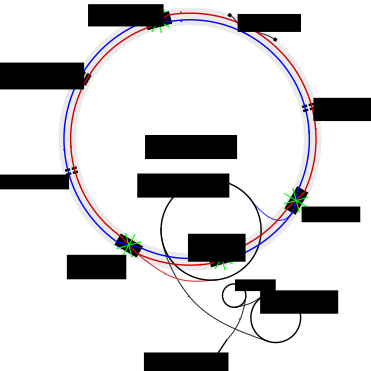
\includegraphics[width=0.8\textwidth]{lhc}
    \caption{Schematic illustration of the \acs{CERN} accelerator complex. Shown are \ac{LINAC} 2, the \ac{PSB}, \ac{PS}, \ac{SPS} and the LHC with its four experiments \acs{CMS}, \acs{ATLAS}, \acs{LHCb} and \acs{ALICE}. The accelerator sizes and positions are not to scale\cite{Ley:CERNAccelerators,Caron:LHCLayout
    ,DeMelis:CERNacceleratorcomplex}.}
    \label{fig:LHC}
\end{figure}

This work will focus on the \ac{CMS} experiment, which will be discussed in the next sections.

\section{The Compact Muon Solenoid}
The \ac{CMS} detector consists of multiple particle detector subsystems surrounding the interaction point.
Its goal is to measure outgoing particles created at proton-proton collisions.
The observed properties include particle type, direction, momentum, energy and charge. Each of the detector subsystems are dedicated to measuring one or more of these characteristics. The subsystems are read out electronically and the data are later analyzed on a computing grid.

An overview of the detector can be seen in \fref{fig:CMS_slice}. The discussion of the detector subsystems in the following sections is based on \cite{Chatrchyan:CMSexperimentCERN} if not explicitly stated otherwise.

\begin{figure}
    \centering
    \raisebox{0.31\height}{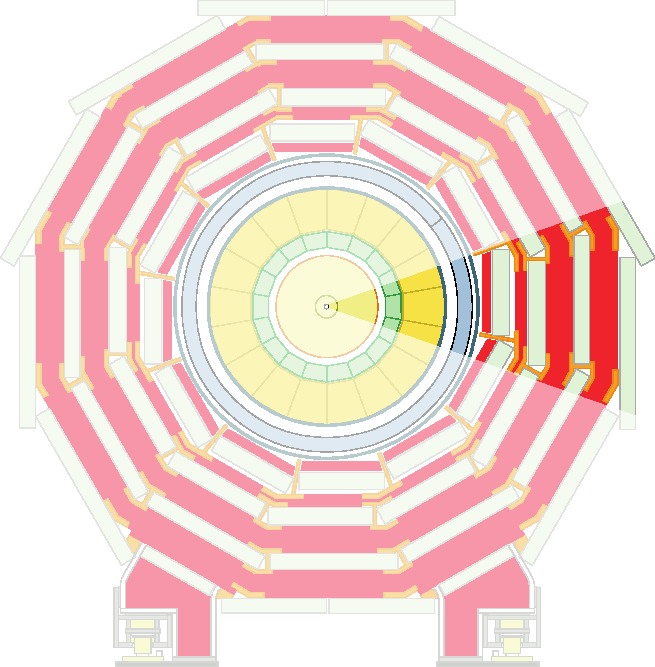
\includegraphics[width=0.3\textwidth]{cms_slice_context}}
    \hspace{0.02\textwidth}
    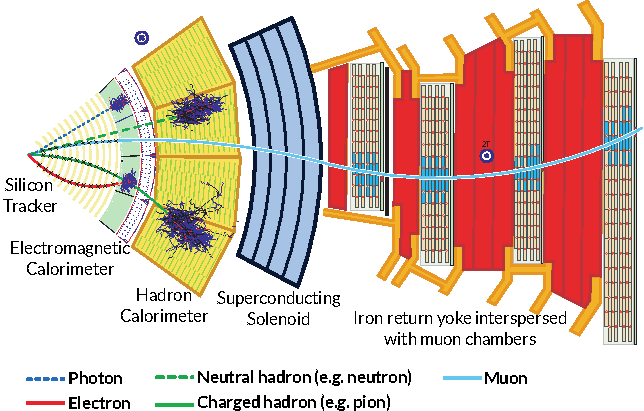
\includegraphics[width=0.65\textwidth]{cms_slice}
    \caption{Slice through the CMS detector barrel. From left to right the following subsystems are drawn: the silicon tracker, the electromagnetic and hadron calorimeter, the superconducting solenoid coil, and the iron return yoke with the muon chambers. The solid lines represent charged particles which are bend due to the magnetic field\cite[modified]{Davis:CMSSlice}.}
    \label{fig:CMS_slice}
\end{figure}

\subsection{Detector Geometry}
In a region starting at \SI{23}{\m} before the detector, both beam pipes are united\cite{Evans:LHCMachine}. The proton groups traveling in opposite directions share the same beam pipe, which defines the $z$-axis of the detector coordinate system. The collisions occur at $z = 0$.
The detector forms a barrel around the beam pipe. The barrel is subdivided into seven slices: five evenly sized \emph{wheels} and one so-called \emph{endcap} on each open side of the barrel. The central wheel is centered at $z = 0$.
Detector layers in the wheels are mostly arranged in a cylindrical manner around the beam pipes, while the layers in the endcaps are mounted orthogonally to the beam pipe.

\subsection{Bunch Crossings and Pile-Up}
\label{sec:pileup}

For acceleration reasons, protons in the \ac{LHC} are grouped into packets called \emph{bunches}. At the interaction point, proton bunches from both directions collide every \SI{25}{\nano\second}, defining the so-called \emph{bunch crossing}. During each bunch crossing, multiple proton pairs may interact with each other. This multitude of collisions is called \emph{pile-up effect}.

Similarly, the collision of a single proton pair may result in multiple partons interacting with each other. This ambiguity is resolved by only analyzing the interaction with the highest momentum transfer, called \emph{hard interaction}. Other interactions contribute to the so-called \emph{underlying event}.

\subsection{Subsystems}
\subsubsection{Inner Tracking System}
The \emph{inner tracking system} is used for precise measurements of direction and curvature of charged particles. 
It is composed of silicon semiconductor pixel layers surrounded by strip modules.

Each pixel cell consists of a silicon semiconductor in reverse bias direction. Charged particles passing through the semiconductor induce ionization and thus allow small currents to flow. These currents are amplified and read out by dedicated electronics. There are about \num{66} million pixel cells, each with a size of $\SI{100}{\micro\meter} \times \SI{150}{\micro\meter}$, allowing for a high spacial resolution.

The strip modules function similarly to the pixel cells. For reduced production costs, typical cell sizes are $\SI{10}{\centi\meter} \times \SI{80}{\micro\meter}$. There are \num{24244} silicon strips in the tracker.

A very high spacial resolution around the interaction point is necessary for finding the origin of decay products. This is achieved by tracing the particle tracks back to the location of their parent particles. The information is later used to discard particle tracks originating in pile-up  events or the underlying event (see \fref{sec:pileup}), as well as for identifying decays of \PB-mesons (see \fref{sec:b_tagging}).

\subsubsection{Electromagnetic Calorimeter}
\label{sec:ecal}
The goal of the \acfi{ECAL} is to measure the energy of outgoing electrons, positrons and photons. 

It consists of dense, transparent lead tungstate ($\textup{PbWO}_4$) crystals. Within these crystals, high energetic electrons and photons cause electromagnetic cascades: Electrons emit photons in the process of bremsstrahlung, while photons convert to electron-positron pairs in the process of pair-production.
This leads to large numbers of lower-energy electrons and photons, until the electron energy loss is dominated by ionization losses and the photon energy is below the pair-production threshold of $2 \si{\electronmass} = \SI{1022}{\keV}$.
Low energetic photons and those emitted by ionization or excitation are eventually registered using photodiodes. The initial particle energy is calculated from the light yield.\cite{ParticleDataGroup:ReviewParticlePhysics}.

As long as the cascade does not leak through the photodetectors, the achieved energy resolution for photons is about \SI{1}{\percent}.\todo{electrons, quelle}

\subsubsection{Hadron Calorimeter}
The \acfi{HCAL} measures the energy of hadrons produced during the collision. 

It is designed as a sampling calorimeter with alternating layers of brass absorbers and plastic scintillator tiles. Hadrons passing through the calorimeter interact with nuclei of the denser brass absorbers. During collisions, secondary charged (\Pgppm, \Pproton, ...) as well as neutral hadrons (\Pgpz, \Peta, ...) are produced. The charged secondaries cause electromagnetic radiation via ionization while the neutral particles decay into photons, which themselves cause electromagnetic showers (see \fref{sec:ecal}).

The charged particles from electromagnetic showers are detected via scintillation. In the plastic scintillators, passage of charged particles induce emission of optical photons. These are guided to photodiodes using wavelength-shifting fibers. The fiber material suppresses Cherenkov light and do not act as scintillators themselves.\cite{ParticleDataGroup:ReviewParticlePhysics}.

Because of the short radiation lengths in the absorber material, sampling calorimeters are more space efficient than homogeneous calorimeters.
However, as some of the energy is deposited within the absorber material, the total shower energy can only be estimated from the scintillation light.

Similarly to the electromagnetic calorimeter, a high resolution can be achieved only as long as the showers do not leak through the calorimeter.

\subsubsection{Solenoid Magnet}
The \ac{CMS} solenoid magnet is designed to deliver a magnetic field strength of \SI{4}{\tesla}. This is achieved by cooling the \SI{220}{\tonne} cold mass to \SI{4.6}{\kelvin}, such that the NbTi wires become superconducting and the current can reach up to \SI{19.5}{\kilo\ampere}.
The magnet surrounds the calorimeters and has a diameter of \SI{6}{\meter}. Within the coil, the magnetic field is approximately uniform with the field lines being parallel to the beam pipe. Outside, the magnetic field lines are closed by an iron yoke, which is interspersed with the muon system.

Particles passing the field are subject to the Lorentz force which subsequently bends their tracks into circular curvatures. This effect allows to distinguish between charged and neutral particles and enables measurement of particle momenta independently of their energy.

\subsubsection{Muon System}
The goal of the muon system is to detect muons and measure their tracks, from which the muon momenta are calculated.

Because of their high mass compared to electrons, muons are less affected by the electromagnetic fields within matter, reducing their radiative losses. This makes them the only detectable particles to pass through all inner detector subsystems as well as the solenoid coil.
For this reason, the muon system is the outermost part of the detector. It surrounds the solenoid coil and consists of \emph{drift tubes} (\acsu{DT}s) and \emph{cathode strip chambers} (\acsu{CSC}s). 

Drift tubes have a length of about \SI{2}{\meter} and a cross section of $\SI{13}{\milli\meter} \times \SI{42}{\milli\meter}$. In the center of each tube, there is an anode wire. Between the wire and the tube walls there is a high electric potential. Additionally, the tubes are filled with a gas mixture. 
As the charged muons pass through the gas, they ionize a few of the gas atoms. The released electrons accelerate along the electric field lines and induce an avalanche of secondary ionizations. Eventually, the accumulated charges are deposited in the anode wires and are measurable as current spike\cite{ParticleDataGroup:ReviewParticlePhysics}.

From the amount of deposited charge and timing measurements, a spacial resolution of less than \SI{250}{\micro\meter} can be achieved across each chamber. However, determining the location in the wire direction is not possible with this arrangement.

In the endcap region, the muon system consists of cathode strip chambers instead of drift tubes. \acp{CSC} work similarly to drift tubes, but instead of having a single cathode at the chamber walls, they contain multiple cathode strips, which are aligned orthogonally to the wires and read out separately.
The advantage of measuring all three dimensions makes them suited for use in the endcap regions where the magnetic field is not uniform. 

\todo{RPCs?}

\subsection{Triggering}
As mentioned in \fref{sec:pileup}, the \ac{LHC} delivers collisions about every \SI{25}{\nano\second}, resulting in around \num{40} million events per second. Even with a raw event size of about \SI{1}{\mega\byte}, storing all events would require a bandwidth of \SI{40}{\tera\byte\per\second}. Currently, there is no technology capable of this task, especially considering the outer circumstances such as irradiation and the strong magnetic field.

Thus, the rate of events accepted for storage and analysis has to be drastically reduced. This is the task of the \emph{triggering system}. Based on the physics content, statistics and bandwidth restrictions, triggers decide whether or not to store an event to disk.

Triggering is implemented in a two step process: First, the \acfi{L1} trigger is consulted. It is implemented in dedicated hardware and uses information from the calorimeters and the muon system to reject low-energetic events. Events passing \ac{L1} will be read out, temporarily stored and further evaluated by the \acfi{HLT}. The \ac{HLT} is implemented in software and running on computers next to the detector cavern. It has access to the full detector information to decide whether an event is eventually stored or rejected.

\subsection{The Computing Grid}
Reconstruction and analyses are ran on the stored events. For this purpose, \ac{CERN} maintains several server farms, organized within the \acfi{WLCG} project.

The facilities are organized in layers called \emph{tiers}. Tier 0 is the \ac{CERN} data center in Geneva. It store raw data and performs initial reconstruction. The data are then distributed to tier 1 computing centers. There are currently 13 tier 1 centers worldwide. They perform further processing on the data and distribute it to tier 3 facilities.

Most of the 155 tier 3 computing centers belong to universities and other scientific institutes. They produce \ac{MC} simulations and perform scientific analyses. One of these tier 3 centers is operated at the physics department of the RWTH Aachen University, currently providing around \num{5200} processing cores and \SI{3}{\peta\byte} of storage. 

\todo{quelle}
% https://home.cern/about/computing/grid-system-tiers
% http://www.institut3b.physik.rwth-aachen.de/cms/ParticlePhysics3B/Forschung/~gbvf/GRID-Computing/


% !TeX spellcheck = en_US
% !TeX encoding = UTF-8
% !TeX root = ../document.tex

\chapter{Event and Object Selection}

\section{Event Selection}
\subsection{Triggers}
\subsection{MET-Filters}


\section{Object Selection}
\subsection{Offline Reconstruction}
\subsection{Identification}
\subsection{b/t-Tagging}

% !TeX spellcheck = en_US
% !TeX encoding = UTF-8
% !TeX root = ../document.tex

\chapter{Datasets}
\section{Monte-Carlo Simulations}
The \ac{MUSiC} analysis aims to search for deviations in a large number of final states and a wide kinematic phase space. Deviations are expected in any area under investigation and therefore there is no signal-free region that could be used for validation or fine tuning. Thus, we avoid data-driven methods as much as possible and rely on theoretical predictions in form of \acl{MC} simulations.

The \ac{MC} simulation is performed on an event-by-event basis. Each event is generated in multiple steps: First, the distribution of proton momentum between partons is simulated. This is done by drawing pseudo-random numbers according to probability distributions related to the empirically measured \emph{parton density functions}.
Afterwards, the hard scattering process is simulated. Similarly as with the momentum distribution, different scenarios are are possible, each with a probability corresponding to the predicted scattering probability. In the second step, parton showering and hadronization is applied: Since the required higher order terms of \ac{QCD} cannot be computed exactly, several parametrized models are used to simulate the formation of hadrons from quarks and gluons. In the last step, the detector response is simulated, also using parametrized interactions of the final state particles with detector components.

In practice, events of different physics processes are simulated in separate sets, so-called \emph{samples}. 
Additionally, some samples only contain events within a certain \pT or mass range. This is done in order to provide a low statistical uncertainty in the tails of steeply falling distributions.

In order to have consistent and validated samples for all \ac{CMS} analyses, the \ac{MC} samples are generated centrally by \ac{CMS} on the \ac{WLCG}.

In addition to weight assigned by generators, each event is assigned a further weight during the analysis. It is computed from the expected cross section, an expected higher order correction factor ($k$-factor) and the luminosity. 
Additionally, events are reweighted to compensate for difference pileup simulation between expectation and data. 
The expected event yield with certain properties can now be obtained by summing the weights of the desired events.

Within this thesis, various luminosity scenarios are analyzed. We did not generate additional \ac{MC} events for each scenario, instead the events are scaled to the described luminosity with the method mentioned above. This allows for a direct comparison ignoring hardware changes made to the detector between the data taking periods in 2015 and 2016.


\subsection{Standard Model}

\newcommand{\genAM}{\textsc{MadGraph\_aMC@NLO}\xspace}
\newcommand{\genBM}{\textsc{BlackMax}\xspace}
\newcommand{\genCA}{\textsc{CalcHEP}\xspace}
\newcommand{\genMG}{\textsc{MadGraph~5}\xspace}
\newcommand{\genPH}{\textsc{Powheg}\xspace}
\newcommand{\genPY}{\textsc{Pythia~8}\xspace}
\newcommand{\genQBH}{\textsc{QBH~2.0}\xspace}
\newcommand{\genSP}{\textsc{Sherpa}\xspace}
\newcommand{\genMCFM}{\textsc{MCFM}\xspace}

\newcommand{\genGEANT}{Geant~4\xspace}

The \ac{SM} samples used by \ac{MUSiC} are produced with the following generator applications: \genMG\cite{Alwall:MadGraph5}, \genSP\cite{Gleisberg:EventgenerationSHERPA}, \genPH\cite{Frixione:MatchingNLOQCDa,Alioli:generalframeworkimplementing}, \genAM\cite{Alwall:automatedcomputationtreea}, \genMCFM\cite{Campbell:Vectorbosonpaira} and \genPY\cite{Sjoestrand:BriefIntroductionPYTHIA}. For the generators \genMG, \genPH, \genAM and \genMCFM, the subsequent hadronization is applied separately using \genPY.
The detector response is simulated with \genGEANT \cite{Agostinelli:GEANT4asimulationtoolkit}.

The full list of used \ac{MC} samples can be found in \fref{app:mc_datasets}.

\subsection{Signal Samples}
The signal study uses the same set of signal samples as the corresponding dedicated analyses \cite{CMS:CMS-PAS-EXO-16-001,CMS:CMS-PAS-EXO-15-007,CMS:CMS-PAS-EXO-16-002,CMSCollaboration:SearchesWbosons}. This makes results comparable and also allows reusing central production and reconstruction by \ac{CMS}. The mass points are chosen to cover a broad range including the resulting limits set by the dedicated analyses. However, since the automated search has to be re-run for each signal sample, computation time limits the amount of samples analyzed.
\begin{itemize}
    \item For the \ac{QBH} model, the \acf{ADD} model with $n = 4$ extra dimensions is analyzed. The chosen mass points $M$ are \SI{1}{\TeV}, \SI{2}{\TeV}, \SI{3}{\TeV}, \SI{4}{\TeV} and \SI{5}{\TeV}. The events are simulated by the \genQBH\cite{Gingrich:MonteCarloevent} generator.
    
    \item In the black hole study, we consider the case of a non-rotating black hole. The fundamental Planck mass is set to $M_\text{D} = \SI{4}{\TeV}$ with $n = 6$ extra dimensions. This choice corresponds to the benchmark result published in \cite{CMS:CMS-PAS-EXO-15-007}. The black hole mass is varied between \SI{6}{\TeV}, \SI{7}{\TeV}, \SI{8}{\TeV}, \SI{9}{\TeV}, \SI{10}{\TeV}. The \ac{MC} generator used for the model is \genBM\cite{Dai:BlackMaxblackhole}.
    
    \item For the Seesaw-TypeIII samples, only the mass points $M_\Sigma = \SI{380}{\GeV}$ and $M_\Sigma = \SI{500}{\GeV}$  are tested. The samples are generated with \genAM\cite{Alwall:automatedcomputationtreea}.
    
    \item The \PWprime model is tested for \PWprime masses of \SI{3}{\TeV}, \SI{4}{\TeV}, \SI{5}{\TeV}. The branching ratio of $\PWprime \to \Ptop \Pbottom$ is set to 1. This sample uses the \genCA\cite{Belyaev:CalcHEP34collider} generator.
\end{itemize}
Again, where necessary, hadronization is applied using \genPY and the detector response is simulated with \genGEANT.

% !TeX spellcheck = en_US
% !TeX encoding = UTF-8
% !TeX root = ../document.tex

\chapter{Model Unspecific Search}

\section{Motivation}
A collision at an energy of \SI{13}{\TeV} can create a large amount of different particles. Solely by combinatorics, it follows that a lot of different final states are accessible.

Most dedicated searches tend to focus on one or a few final states that represent the signature of the theory under investigation. This leaves many final states not examined, either because of the complexity of the final state or because there is no analysis group currently working on a corresponding theory.

One of the goals of the model unspecific search is to gain knowledge from these additional final states. Additionally, the model unspecific search aims to obtain a global interpretation of the agreement between simulation and observed data across a broad range of final states.

\section{Previous Works}
The approach of a model unspecific search is not a new concept: In 1998, a note about an unspecific search has been written at the L3 experiment (\ac{LEP})\cite{Hebbeker:GlobalComparisonL3}, and in 2004, a similar approach has been applied to data of the D0-experiment at the Tevatron proton-antiproton collider at Fermilab\cite{Biallass:ModelIndependentSearch}.

At \ac{CMS}, the analysis has been developed and regularly applied to observed data since 2009\cite{Schmitz:ModelUnspecificSearch,Hof:ImplementationModelIndependent,Dietz-Laursonn:ModelUnspecificSearch,Olschewski:StudyAlternativeStatistical,Brodski:ModelUnspecificSearch,Pieta:MUSiCModelUnspecific,Papacz:ModelUnspecificSearch,Albert:ExtensionModelUnspecific,Roemer:ModelUnspecificSearch} \todo{Jonas' Arbeit, Debby und Simon?}. 
This thesis bases on the most recent implementation of the \ac{MUSiC} analysis.\todo{ok so?}

Very recently, the \ac{ATLAS} collaboration published a conference note analyzing \SI{3.2}{\per\femto\barn} of \ac{LHC} data at $\sqrt{s} = \SI{13}{\TeV}$ using a similar model-independent search \cite{ATLAS:ATLAS-CONF-2017-001}. 

\section{Procedure}
The input to the \ac{MUSiC} analysis are reconstructed events of observed as well as simulated data, which have been centrally reconstructed by the \ac{CMS} collaboration.
As first step of the \ac{MUSiC} analysis, requirements on events and physics objects are applied, discarding unwanted events and extracting objects for the \ac{MUSiC} analysis (see \fref{chap:selection}).
Afterwards, each event is classified sorted into so-called \emph{event classes}, sets of events that share the same final state.
For each event class, the kinematic variables of each event are calculated and \emph{kinematic distributions} are aggregated.
Up to this point, the same procedure is applied to simulated data and observed data.
Subsequently, an automated search algorithms finds the largest deviation between data and simulation within each kinematic distribution of each event class. Afterwards, the global significance of each deviation is estimated from Standard-Model only simulations.

\section{Event Classes}
An event class is a set of events sharing the same final state. The final state is indicated by the name of the event class: All events in the class named \eventclass{2\Pe + 1\Pmu}, for example, contain two electrons and one muon in the final state.

There are three types of event classes: \emph{exclusive}, \emph{inclusive} and \emph{jet inclusive}.

Events in the exclusive event classes contain exactly the indicated (and no additional) particles in their final state. Each event thus belongs to exactly one exclusive event class.

Inclusive event classes are denoted with the suffix "\eventclass{+ X}" in the name (for example \eventclass{2\Pe + 1\Pmu + X}). Their final state contains the explicitly stated particles plus any additional ones. Each event can be assigned any number of inclusive event classes. One advantage of this procedure is a larger number of events per class which can be beneficial \todo{for what?}. However, the correct combination of statistical results across multiple inclusive event classes is not trivial.

Jet inclusive event classes are denoted with the suffix "\eventclass{+ Njets}" in the event class name (e.g. \eventclass{2 \Pe + 1\Pmu + Njets}). Events contained in a jet inclusive event class may contain any number of jets in addition to the explicitly stated objects. This increases the number of events per class, as effects like initial or final state radiation are ignored, leading to reduced statistical uncertainties.

In any case, the kinematic variables are only calculated from the objects explicitly stated in the class name, in our example two electrons and one muon.


\section{Particle Types}
Not all particle types that can be identified by the experiment are used within the classification. Instead, \ac{MUSiC} focuses on a set of five particle types which can be measured most precisely.
Additionally, certain selection criteria are imposed onto each particle in the final state to obtain an unambiguous final state.
The particle types and identification criteria are described in the following sections.

big picture
why ids (why not just reco)
general id criteria: pt, tracks, shower


\subsection{Electrons}



\subsection{Muons}

\subsection{Photons}

\subsection{Jets}

\subsection{Missing Transverse Energy}

\subsection{Possible Extensions}
The analysis can be extended to identify more particle types by their decay products, called \emph{tagging}. Possible tagging choices are \Pqb-tagging, \Ptau-tagging or \PZ-tagging.
This thesis will investigate the increase of sensitivity using \Pqb-tagging. The method is further described in chapter \todo{ref}.

\section{Transverse Momentum and Transverse Energy}
\todo{context?}

Interaction cross sections are often dependent on the amount of momentum involved. In t-channel diagrams, the entire momentum transfer can be measured by calculating the combined invariant mass of decay products.
In order to achieve this goal, one must know all four components of the momentum of all created particles. If the final state contains neutrinos, which are not detectable by the detector, this is not achievable.

In other experiments like \ac{LEP}, one could use conservation of momentum and the known momentum of colliding particles to reconstruct the neutrino four-momentum and the momentum transfer. At the \ac{LHC} this is also impossible: The total proton momentum is distributed unevenly between the constituent quarks and gluons and thus the momentum involved in a collision is only known up to statistical probability.

The mitigation pursued at \ac{CMS} is to only regard kinematics in the transverse plane, orthogonally to the beam pipe. Projection of the kinematic (three-)momentum onto the transverse plane gives the so-called \emph{transverse momentum} \pT.

An additional property of the transverse momentum is that it can be directly observed: Since the magnetic field lines are parallel to the beam direction, the Lorentz force only acts in the transverse plane, allowing direct observation of the transverse momentum.

Assuming $p_x$, $p_y$, $E$ and $m$ can be observed directly (e.g. via track curvature) or indirectly (e.g. via particle identification), we can define the transverse momentum and transverse energy as follows:
\begin{align*}
\vec{p}_T &\defeq \left( p_x, p_y, 0 \right)^T  \\
\vec{E}_T &\defeq E \frac{\vec{p}_T}{\abs{\vec{p}}} = \frac{\vec{p}_T}{\sqrt{1-\left(m/E\right)^2}}
\end{align*}

Note that in the approximation of massless ($m \approx 0$) particles: $\vec{p}_T = \vec{E}_T$. % $ = \vec{M}_T$.

%cross sections are dependent of momentum transfer
%in t-channel diagrams: momentum transfer is invariant mass of created particles
%calculate inv mass from 4-vectors of all particles
%problem if neutrinos are produced
%other approaches (both done at LEP): control COM energy of interaction precisely, or use momentum conservation to reconstruct neutrino 4-momentum
%problem: energy of and initial momentum in beam direction unknown because of partons
%mitigation: use knowledge about momentum in transverse plane, calculate momenta and energy there
%pT has additional advantages: measured directly (magnetic field) and is invariant regarding pdfs/z-boosts

\section{Kinematic Variables and Distributions}
For each event, the \ac{MUSiC} classification calculates three scalar variables: the sum of transverse momenta, the invariant mass and the missing transverse energy.

The sum of transverse momenta is the most directly observed variable. For charged particles, the transverse momentum can be deduced directly from the curvature within the magnetic field. The transverse momentum is invariant against Lorentz-boosts in the $z$-direction from the uneven momentum distribution within the proton.
In the following, the sum of transverse momenta will be denoted with \sumpT and defined as follows:
\begin{equation}
    \sumpT \defeq \sum_i \abs{\vec{p}_{T,i}} 
\end{equation}

The invariant mass is, as mentioned before, very sensitive to resonances in the t-channel. If the event class definition contains missing transversal energy passing the selection criteria, the invariant mass will not be computed, instead the transversal mass is used. The variables are denoted with \Minv and \MT respectively and defined as:
\begin{align}
    \Minv &\defeq \sqrt{\left(\sum_i E_i\right)^2 - \left(\sum_i \vec{p}_i\right)^2} \\
    \MT &\defeq \sqrt{\left(\sum_i E_{T,i}\right)^2 - \left(\sum_i \vec{p}_{T,i}\right)^2}     
\end{align}

The third kinematic variable is missing transversal energy. This variable is only calculated if the event class definition explicitly contains missing transversal energy.
The variable is denoted with \MET defined as follows:
\begin{equation}
    \MET \defeq \abs{- \sum_i \vec{E}_{T,i}} 
\end{equation}


\section{Search for Deviations}
\label{sec:deviations_search}

\newcommand{\TS}{\ensuremath{\uptheta}\xspace}
\newcommand{\TSmin}{\ensuremath{\theta_\text{min}}\xspace}

After the classification follows an automated search for deviations. The search is performed on each distribution of each event class separately as follows:
First, multiple bins are combined to a \emph{region}, according to the rules in the following section. Then, a test statistic \TS for each region is calculated. The region with the lowest value of \TS, called \TSmin, is selected. This region will be called \acfi{RoI}. 
Subsequently, a global $\ptilde$-value for the region is calculated. This $\ptilde$-value expresses the probability of finding a deviation with $\TS \leq \TSmin$ purely by chance. Details on the procedure can be found in \fref{sec:global_significance}.

\subsection{Search Space}
The search is performed on so-called regions. A region is a set of adjacent bins and is represented by the combined number of expected and observed events as well as a combined uncertainty.

For the \sumpT and \MET kinematic distributions, the minimal number of bins in a region is \num{3}, in order to be insensitive towards narrow deviations from \ac{MC} statistics \todo{explain spikes}.
For a increased sensitivity to resonant deviations, the minimal number of bins in the \Minv and \MT distributions is \num{1}.

An additional criterion on the regions is based on the number of simulated events in a region. If a region shows a lack of simulated events, the test statistic is not computed for this particular region. Since each region (that is not the entire distribution) is embedded in a larger region, regions skipped in this step are still considered. \todo{low stats ausfuerlicher erklaeren?}

The combined number of events and the combined uncertainty for each region is calculated as
\begin{align}
     N_{\text{total},\text{exp}} &= \sum_i N_{i, \text{exp}} \\   
     N_{\text{total},\text{obs}} &= \sum_i N_{i, \text{obs}} \\
     \sigma_\text{total} &= \sqrt{\sum_i \sigma_i^2 + 2 \sum_{i,j} \rho_{i,j}\sigma_i\sigma_j}
\end{align}
where $\rho_{i,j}$ is the correlation coefficient for the uncertainty $\sigma$ between the bins $i$ and $j$.

Some uncertainties, such as the statistical uncertainty on the simulated number of events, are completely uncorrelated between the bins. The correlation coefficient thus is $\rho_{i,j} = 0$ and the total uncertainty is the quadratic sum of the bin uncertainties.

Other uncertainties are correlated between bins. An example for this is the uncertainty on the luminosity measurement, which affects all bins of all distributions the same way. We treat any uncertainty that is assumed to be correlated to some extend as fully correlated ($\rho_{i,j} = 1$) and calculate the combined uncertainty as linear sum. This method possibly overestimates the total uncertainty, in case the correlation coefficient is somewhere between 0 and 1, leading to a lower \todo{(conservative?)} sensitivity.

\subsection{Global Significance}
\label{sec:global_significance}

The goal of the automated search is to find the largest deviation between expected and observed number of events in a region. The size of a deviation is expressed as value of the test statistic \TS. A larger deviation will result in a smaller value of \TS.
The formula for computing \TS will be derived in the next chapter. \todo{mention \TS = local p value?}

From the test statistic, we will calculate a global significance, to which we refer as \ptilde. It expresses the probability of finding a deviation equally large or larger than the observed one somewhere in the distribution, if the expectation were true.

The simplest way of calculating \ptilde would be to first calculate a local $p$-value from the test statistic and then apply a correction factor to it. A suitable correction factor can be estimated using combinatorics, if the possible values of the local $p$-value are uncorrelated. This method is also called \emph{Bonferroni correction}. 

In our case, a purely analytically calculation is not possible because the connected bin regions overlap and thus the local significances are correlated.

Instead, we use a simulation-based approach:
We simulate possible experimental outcomes based on the distribution of expected number of events, and refer to each simulation round as \emph{pseudo-experiment}.
During each pseudo-experiment, we randomly draw a substitute observed distribution from the expected number of events. 

correlated uncerts: shared value of standard gaussian multiplied with local width of uncert
uncorrelated: random from normal distribution
summed up
poissonian draw for quantum-phenomena

\begin{algorithm}
    \caption{Pseudo Experiment}
    \newcommand{\Nobs}{n}
    \newcommand{\Nexp}{N}
    \newcommand{\corr}{corr}    
    \newcommand{\uncorr}{uncorr}
    \newcommand{\x}{x}
        
    \begin{algorithmic}
        \Require $\Nexp_{i=1..n} \gets $ number of events in each bin $i$
        \Require $\corr_{i=1..n,j=0..c} \gets $ correlated uncertainty $j$ in each bin $i$
        \Require $\uncorr_{i=1..n,k=0..u} \gets $ uncorrelated uncertainty $j$ in each bin $i$
        
        \Statex
        
        \ForAll {correlated uncertainty $j$ in distribution}
            \State $\x_j \gets \text{RandNormal}(\mu = 0, \sigma = 1)$
        \EndFor
        
        \ForAll {bin $i$ in distribution}
            \State $\Nobs_i \gets \Nexp_i$
            \ForAll {correlated uncertainty $j$ in bin $i$}
                \State $\Nobs_i \gets \Nobs_i + \x_j \cdot \corr_{i,j}$
            \EndFor
            \ForAll {uncorrelated uncertainty $k$ in bin $i$}
                \State $\Nobs_i \gets \Nobs_i + \text{RandNormal}(\mu = 0, \sigma = \uncorr_{i,k})$
            \EndFor
            \State $\Nobs_i \gets \text{RandPoisson}(\Nobs_i)$
        \EndFor
    \end{algorithmic}
\end{algorithm}

The recipe for each pseudo-experiment is as follows:

Let $\sigma_u(i,j)$ be the value of the uncorrelated uncertainty and $\sigma_v(i,j)$ the value of a correlated uncertainty with index $j$ in bin $i$. Further, let $\ev{N_{i}}$ be the expected number of events in bin $i$.



Start by simulating a pseudo-true value for correlated uncertainties since this impacts all bins differently, we choose from a standard normal distribution $\mathcal{N}$:
\begin{equation}
    v_j \sim \mathcal{N}(\mu = 0, \sigma = 1)
\end{equation}

The impact factor for uncorrelated uncertainties is calculated separately for each bin:
\begin{equation}
    u_{i,j} \sim \mathcal{N}(\mu = 0, \sigma = 1) 
\end{equation}

\begin{equation}
    \ev{n_i} = \ev{N_i} + \sum_j^{\text{uncorrelated}} u_{i,k} \sigma_u(i,j) + \sum_k^{\text{correlated}} v_{i,k} \sigma_v(i,k)
\end{equation}

Finally draw an integer value from the Poisson distribution $\mathcal{P}$ with the expectation value $\ev{n_i}$.
\begin{equation}
    n_\text{obs} \sim \mathcal{P}(\lambda = \ev{n_i})
\end{equation}


For each \emph{pseudo-experiment}, we draw a random number of events for each bin of the distribution simultaneously. The number is drawn from the probability distribution caused by systematical and statistical uncertainty around \ac{SM} expectation value. 


 of \emph{pseudo-experiments}: For each bin of the distribution, a random number is drawn from the probability distribution caused by systematical and statistical uncertainty on the \ac{SM} expectation value. The resulting \emph{pseudo-distribution} is subsequently again compared to the expectation using the described search algorithm, yielding a local significance value \TS for each pseudo-experiment.
The step of randomly generating a distribution and searching for a deviation is repeated \num{e5} to \num{e6} \todo{number} times.

Finally, the global \ptilde-value is calculated by determining the rate of pseudo-experiments where $\TS_{\text{random}, \text{min}} < \TS_{\text{obs}, \text{min}}$. Note that the definition of a $p$-value ("probability to find a deviation equally large or larger as the observed one by chance") corresponds directly to the computed \ptilde-value in the frequentist interpretation.

%Within the (statistical and systematical) uncertainty distribution of the Standard Model  
%The statistical nature of the Standard-Model is simulated by randomly choosing values for the observed number of events in each bin.
%The probabilities of observing deviations are correlated between overlapping regions. 
%Since the regions' overlap, the regions are correlated. Thus, the probabilities of observing deviations by chance are correlated between overlapping regions.
%assess the significance of a deviation, expressed as probability to observe a deviation the same as or more extreme just by chance (given SM) SOMEWHERE in the distribution
%procedure also known as Bonferroni correction
%correction factor cannot be calculated analytically because of correlations between regions
%idea: pseudo-experiment, simulate circumstances using SM only, count more-extreme values, interpret fraction as probability (frequentist  approach)
%problem: need measure for "extremity" of deviation (-> also used for finding RoI)

\subsection{Test Statistic}
\label{sec:test_statistic}

measure "extremity" of deviation (-> for finding RoI as well as global correction)

choice is ambiguous

choice: value interpretable as probability for local deviation

back to definition: sum of probabilities of more extreme events

start using Poissonian probability
include Gaussian prior: either normal or log normal


most of the systematic uncertainties scale number of events in a region rather than a constant shift. examples: lumi, xsec, PDF, ID efficiency, misID


The total number of events is thus scaled by an unknown factor $X$, which is a random variable that emerges as product of multiple other random variables $x_i$.
In the following section, we will derive how $X$ is distributed.

We begin with rewriting the product in terms of a sum within an exponential distribution:
\begin{equation}
    X = \prod_i x_i = \prod_i \exp(\ln(x_i)) = \exp(\sum_i \ln(x_i))
\end{equation}
$\ln(x_i)$ is a random variable, and the central limit theorem implies that the sum is distributed according to the normal distribution.
\begin{equation}
    Y \defeq \sum_i \ln(x_i) \Rightarrow X = \exp(Y) \text{ and } f_Y(y) = \frac{1}{\sqrt{2\pi}\sigma} \exp(-\frac{1}{2}\left(\frac{y-\mu}{\sigma}\right)^2)
\end{equation}
After defining $Y$ as the normally distributed variable with the probability density $f_Y(y)$, we introduce a new unknown probability density function $g_X(x)$:
\begin{equation}
    f_Y(y) \: \dd y \eqdef g_X(x) \: \dd x 
\end{equation}
Finally, we can insert all definitions, calculate the derivative and write the distribution function dependent of $x$:
\begin{align}
    g_X(x) &= f_Y(y) \: \dv{y}{x} \\
    &= f_Y(\ln{x}) \: \dv{\ln{x}}{x} \\
    &= f_Y(\ln{x}) \: \frac{1}{\abs{x}} \\
    &= \frac{1}{\sqrt{2\pi}\sigma\abs{x}} \exp(-\frac{1}{2}\left(\frac{\ln{x}-\mu}{\sigma}\right)^2)
\end{align}
The result is known as \emph{log-normal distribution} and is the probability density function of a product of random variables.

By performing two substitutions, we obtain a parametrization with a more meaningful interpretation:
\begin{equation}
    \sigma \rightarrow \ln{k} \text{ and } \mu \rightarrow \ln{x_0}
\end{equation}
\begin{equation}
    g_X(x) = \frac{1}{\sqrt{2\pi}\abs{x}\ln{k}} \exp(-\frac{1}{2}\left(\frac{\ln(x/x_0)}{\ln{k}}\right)^2)
\end{equation}

\todo{explain meaning of parameters}

\subsection{Treatment of Regions With Too Few Simulated Events}


\subsection{Look-Elsewhere-Effects}
\subsubsection{Regions}
corrected using global significance 

\subsubsection{Classes}
\subsubsection{Distributions}

\section{Implementation}
\subsection{Software Environment}
CMSSW, ROOT, Python/C++

\subsection{Analysis Framework}
Skimming, Pxl, TAPAS, MUSiC

\subsection{MUSiC Workflow}

\subsection{Automation}
\begin{figure}
    \centering
    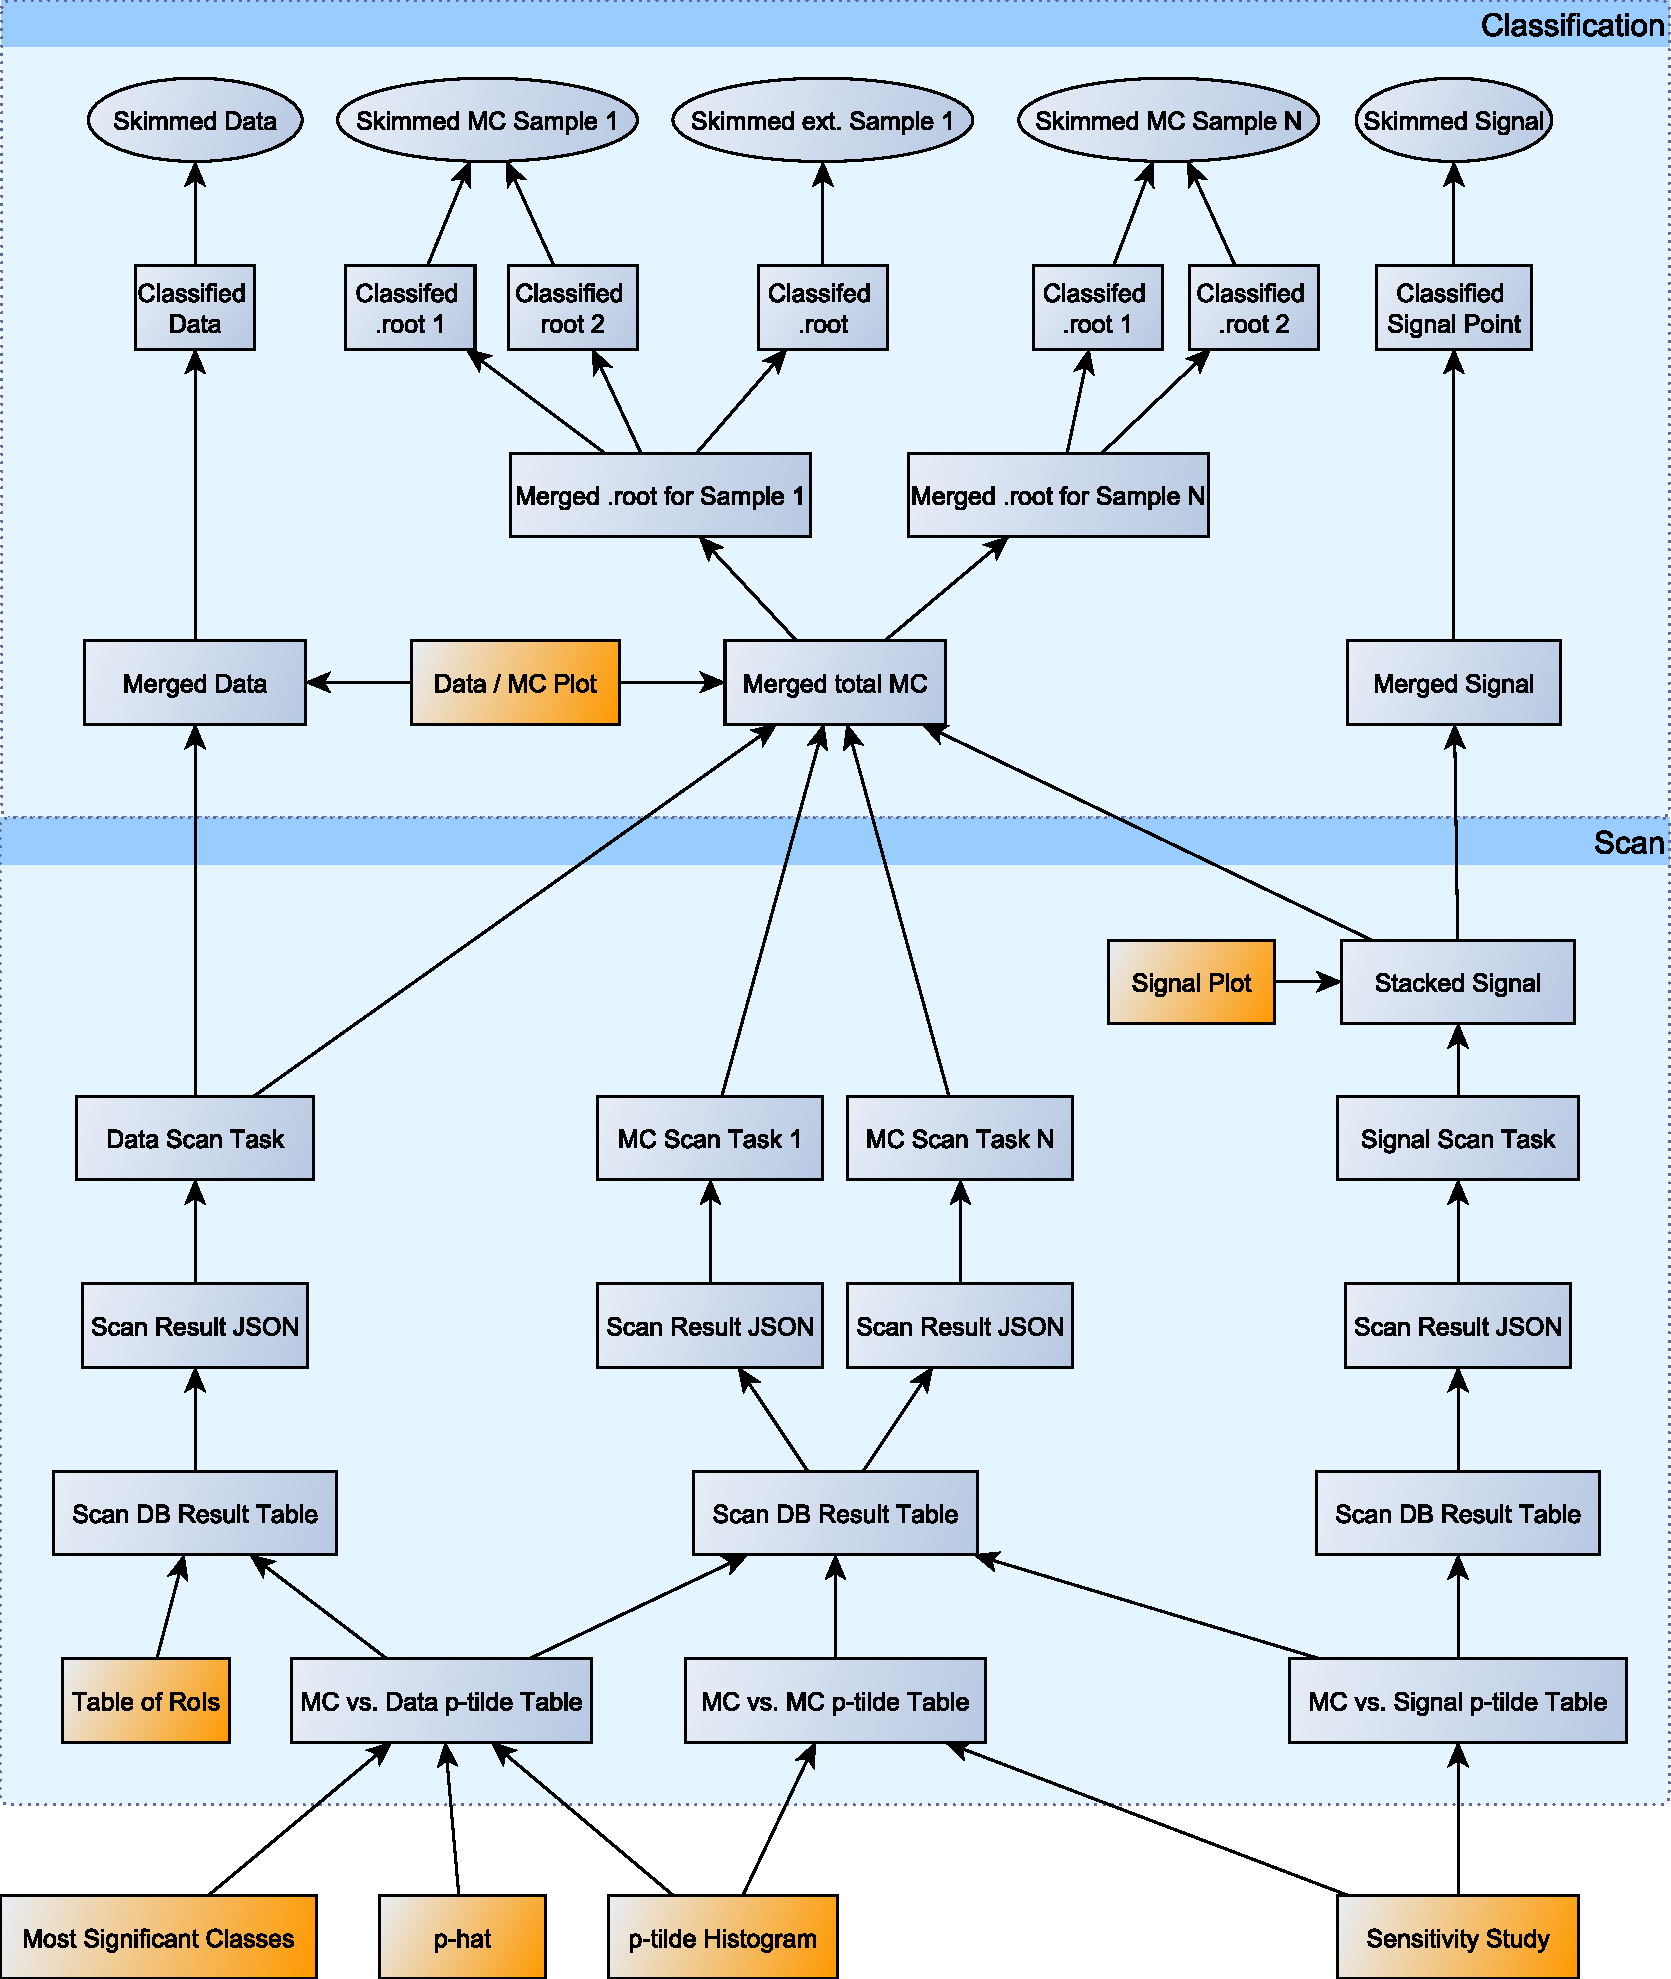
\includegraphics[width=\textwidth]{../music-workflow}
    \vspace{0.5em}
    \caption{Implementation of the MUSiC-Workflow. Using the Luigi-Automation Framework, these steps are performed on demand.}
    \label{fig:music_workflow}
\end{figure}

Luigi
% !TeX spellcheck = en_US
% !TeX encoding = UTF-8
% !TeX root = ../document.tex

\chapter{Conclusion}
The \acf{MUSiC} is a complex analysis with the ultimate goal to discover new physics in \ac{LHC} data. It consists of a multitude of algorithms and parameters which have to be implemented and optimized by the analyst. This process is usually guided by physical intuition and manual inspection of analysis results. However, it is important to regularly perform a systematic reevaluation of the state of the analysis and  study its discovery potential.
In this thesis, the framework for such a study has been refined and subsequently applied to existing features as well as newly introduced extensions of the analysis.

Among the evaluated features was the inclusion of \Pqb-tagged jets as dedicated physics objects, which has not been part of the analysis since the increase in collision energy to $\sqrt{s} = \SI{13}{\TeV}$ in 2015. Although the increase in sensitivity could not be explicitly shown on the provided benchmark models, the feature is predicted to increase sensitivity towards new physics and therefore should be further investigated in the future.

On the technical side of the analysis, the complexity of the tool chain has grown. This has motivated employing further automation, through which it was possible to cope with the additional workload posed by the exploration of the multidimensional parameter space.
Additionally, a \acl{LUT} has been implemented and evaluated in order to optimize the performance of the automated search for deviations.

Taking up discussions published in a thesis eight years ago\cite{Schmitz:ModelUnspecificSearch}, the potential of a log-normal prior within the local test statistic has been evaluated. For this purpose, a study of the coverage behavior of both the Gaussian- and log-normal prior has been performed, indicating that the log-normal option features superior coverage properties. However, several difficulties regarding pseudo-experiments with a log-normal prior arise. Possible mitigations have been discussed, and it was decided to maintain using the Gaussian prior with additional constraints on the search space.

Another new feature within the analysis is the computation of a global $p$-value. It allows to quantify deviations within the distribution of \ptilde-values, instead of judging deviations by eye. The feature enables future analysts to observe whether a certain change of a parameter value or the implementation of a new feature increases the sensitivity towards certain benchmark models.

Finally, the sensitivity of the analysis towards four models of new physics has been assessed. These benchmark models have been chosen to cover a wide range of possible signatures of new physics. By combining simulated events of these models with \acl{SM} processes, generating pseudo-experiments and analyzing the resulting distributions with the automated search, the impact of each model on the statistical inference has been evaluated. 
In two instances, the \PWprime and the Seesaw Type-III model,  the sensitivity did not (or barely) suffice to discover the presence of the simulated events. In these cases, a comparison to the dedicated analyses was drawn, yielding several suggestions for features that may increase the sensitivity.
The discovery potential for the two other models, semiclassical and quantum black holes, could successfully be shown. The highest discoverable object masses are in agreement with mass limits from corresponding dedicated analyses.

In the future, I would like to encourage analysts who pursue a model independent analysis approach to regularly reevaluate the sensitivity of their analysis to a wide range of new physics simulations. Furthermore, I would suggest to refine the idea of a global $p$-value and a measure of sensitivity, as informed decisions will help the analysis to remain lean and efficient for discovering new physics.

%automation
%bJets
%LUT
%coverage
%evaluation of lognormal
%phat

\cleardoublepage
\bibliographystyle{CMS}
\bibliography{bibliography,images,theses}

\cleardoublepage
% !TeX spellcheck = en_US
% !TeX encoding = UTF-8
% !TeX root = ../document.tex

\chapter{Glossary of Terms}
\todo{check capitalization}
\begin{acronym}[RPV-SUSYx]
    \setlength{\parskip}{0ex}
    \setlength{\itemsep}{0ex}
    
    % WARNING: Make sure that this is ordered alphabetically, as LateX does not apply any ordering itself!

    \acro{ADD}{Arkani-Hamed-Dimopoulos-Dvali\acroextra{ model}}
    \acro{ALICE}{A Lead Ion Collider Experiment}
    \acro{ATLAS}{ATLAS experiment\acroextra{ orig. A Toroidal LHC Apparatus}}
    \acro{BH}{black hole}
    \acro{CERN}{European Organization for Nuclear Research\acroextra{ (orig. Conseil Européen pour la Recherche Nucléaire)}}
    \acro{CKM}{Cabibbo-Maskawa-Kobayashi\acroextra{ matrix}}
    \acro{CMS}{Compact Muon Solenoid\acroextra{ experiment}}
    \acro{CSC}{cathode strip chamber}
    \acro{CSVv2}{Combined Secondary Vertex version 2\acroextra{ algorithm}}
    \acro{DT}{drift tube}
    \acro{ECAL}{electromagnetic calorimeter}
    \acro{HCAL}{hadron calorimeter}
    \acro{HEEP}{High Energy Electron Pairs\acroextra{ selection criteria}}
    \acro{HLT}{high level trigger}
    \acro{L1}{level-1\acroextra{ trigger}}
    \acro{LEP}{Large Electron Positron Collider}
    \acro{LHCb}{Large Hadron Collider beauty\acroextra{ experiment}}
    \acro{LHC}{Large Hadron Collider}
    \acro{LINAC}{Linear Accelerator}
    \acro{LUT}{Lookup Table}
    \acro{MC}{Monte Carlo\acroextra{ simulation}}
    \acro{MUSiC}{Model Unspecific Search in \acs{CMS}}
    \acro{PF}{Particle-Flow\acroextra{ algorithm}}
    \acro{PS}{Proton Synchrotron}
    \acro{PSB}{Proton Synchrotron Booster}
    \acro{QBH}{quantum black hole}
    \acro{QCD}{quantum chromodynamics}
    \acro{QED}{quantum electrodynamics}
    \acro{QFD}{quantum flavordynamics}
    \acro{RoI}{region of interest}
    %\acro{RPV-SUSY}{R-Parity Violating \acl{SUSY}}
    \acro{RS}{Randall-Sundrum\acroextra{ model}}
    \acro{SM}{Standard Model}
    \acro{SPS}{Super Proton Synchrotron}
    \acro{SSM}{Sequential Standard Model}
    \acro{SUSY}{Supersymmetry}
    \acro{WLCG}{Worldwide LHC Computing Grid\acroextra{ project}}
\end{acronym}

\cleardoublepage
% !TeX spellcheck = en_US
% !TeX encoding = UTF-8
% !TeX root = ../document.tex


\renewcommand\thechapter{A}
\chapter{Appendix}



\cleardoublepage
% !TeX spellcheck = de_DE
% !TeX encoding = UTF-8
% !TeX root = ../document.tex

\thispagestyle{plain}
{\usekomafont{chapter}Danksagung}
\chapterheadendvskip

Diese Masterarbeit wäre nicht möglich gewesen ohne viele Menschen, die mich während des Studiums und der Arbeit unterstützt haben.

Für die Chance, dieses Thema im Rahmen der \ac{MUSiC}-Analyse zu bearbeiten und damit direkt in der Forschung mitzuwirken, für die Unterstützung während der Entwicklung und für die Korrektur der Arbeit danke ich ganz besonders Herrn Professor Thomas Hebbeker.
Des weiteren danke ich Dr.~Arnd Meyer dafür, dass er über viele Jahre einen Überblick über die \ac{MUSiC}-Analyse behalten hat, und mit seinem Expertenwissen bei Fragen zur Seite stand.

Ein ganz besonderer Dank gilt Tobias Pook, als Betreuer, \ac{MUSiC}-Kollege und für das Korrekturlesen der Arbeit. Er hat die Analyse (\ac{MUSiC} bei \SI{13}{\TeV}) mit hervorragendem physikalischen Gespür und Erfahrung in Softwareentwicklung geleitet. Mit seinem Blick für das Essentielle hat er mir stets geholfen, der Arbeit einen Fokus zu geben.

Für die lockere, professionelle Arbeitsatmosphäre danke ich auch der restlichen \ac{MUSiC}-Gruppe, bestehend aus Jonas Roemer, der die \ac{MUSiC}-Klassifikation maßgeblich weiterentwickelt hat, Simon Knutzen, mit dem ich stets komplizierte Statistikfragen diskutieren konnte und Debbie Duchardt, die mit der Analyse des \ac{CMS}-Datensatzes von 2012 eine wichtige Grundlage gesetzt hat.

Ich danke außerdem den anderen Wissenschaftlern der \ac{CMS}-Analysegruppe des III. Physikalischen Instituts A, mit denen ich eng zusammengearbeitet habe. Hierbei sind nicht nur fruchtbare Forschungsergebnisse, sondern auch Freundschaften entstanden.

Professor Martin Erdmann möchte ich nicht nur als Zweitkorrektor dieser Arbeit Dank aussprechen, sondern auch für seinen Einsatz für die Erasmus-Physikstudenten der RWTH. Er hat es mir ermöglicht, zwei Semester meines Masterstudiums an der KTH Royal Institute of Technology in Stockholm zu absolvieren.

Weiterhin möchte ich Dr. Markus Merschmeyer für die Stelle als studentische Hilfskraft danken, durch welche ich meine Kenntnisse der Webentwicklung ausbauen und mein Masterstudium mitfinanzieren konnte.

Zu guter Letzt danke ich meinen Eltern, meinem Bruder und meiner Oma, die mich während meines gesamten Studiums herzlich unterstützt haben, meiner Freundin, die während der stressigeren letzten Monate zu mir stand und meinen Freunden, aus dem Studium, meiner Laufgruppe und dem Aachener Studentenorchester.


\end{document}